\section{Introduction}

% \textcolor{blue}{(Background about the study area)}

\subsection{Sediment contamination in aquatic ecosystems}
% great lakes are important

Rivers and lakes provide essential services for human well-being and biodiversity \cite{Vörösmarty2010GlobalThreats}.
% sediments store many nutrients and contaminants
With intensive industrial and urban development along the shorelines, anthropogenic activities have released 
significant amount of pollutants into the these aquatic ecosystems \cite{DavidAllan2013},
elevating ecological risks as many of these contaminants bioaccumulate in aquatic organisms and eventually enter human 
food chains through fish consumption, posing health risks \cite{Eggleton2004SedDisturbance, USGS_SedimentAssociatedContaminants_2019}.
These ecological and human health risks underscore the urgent need for scientific assessment to inform management strategies \cite{Niemi2004EcologicalIndicators}.

Most of these anthropogenic inputs enter the water through 
both point and non-point sources, carrying two major groups of components: 
nutrients (which are water soluble) and hydrophobic contaminants \cite{Carpenter1998Nonpoint}.
The nutrients (especially phosphorus) are taken up by algae, contributing to eutrophication.
However, hydrophobic chemicals
quickly attach to floating organic particles and settle into the muddy bottom sediments through natural binding processes \cite{DavidAllan2013}.
There they accumulate at the bottom where water meets sediment.
Similar binding and absorption processes turn bottom sediments into
a combined storage area of past pollution \cite{Eggleton2004SedDisturbance, USGS_SedimentAssociatedContaminants_2019, ChiaiaHernandez2022,Burton2002SedQuality}.
The chemicals bounded to sediment particles remain chemically stable for extended periods, effectively preserving pollutant signatures 
and creating a persistent record of contamination events across multiple temporal scales \cite{ChiaiaHernandez2022, Burton2002SedQuality}.
This integrative role establishes sediments as a biogeochemical archive that smooths short-term water column fluctuations,
making sediment contaminant measurements a robust long-term {manifestation} of anthropogenic stress \cite{Karickhoff1984Sorption}.


\subsection{Benthic communities as bioindicators for sediment contamination}
Analysis of the chemical content of sediment is resource-intensive and overlooks bioavailability
(the likelihood that chemicals are transferred to biota),
necessitating complementary indicator approaches \cite{Chapman1990SedimentTriad}.
In most natural ecosystems, individual organisms exhibit physiological and behavioral adjustments under external pressures; 
aquatic benthic macroinvertebrates likewise express stressor-mediated responses that scale to detectable community change \cite{Holling1973}.
Benthic macroinvertebrate assemblages can reflect concentrations of sediment-borne contaminants and habitat conditions \cite{Tampo2021Bioindicators},
rendering them effective bioindicators of sediment contamination levels \cite{Desrosiers2020}.
These responses can be observed through differences in benthic community composition and many attempts to develop indices on small aquatic systems, 
such as small lakes, rivers, and streams, have been shown successful \cite{Cain1992Bioindicators, Archaimbault2010SedimentStreams},
motivating extension to large lakes and great rivers where fewer attempts were made but are promising
 by some successful implementations \cite{Birk2012Methods,Ciborowski2005ZoobenthicIndicators, Reynoldson1995}.

Effective bioindicator development requires balancing ecological relevance with practical applicability.
Ideal taxa should exhibit sensitivity to pollution gradients, maintain wide distribution across environmental gradients within the study area,
and be readily sampled and taxonomically identified \cite{LenatResh2001Taxonomy}.
In large aquatic ecosystems, environmental complexity and heterogeneity present additional challenges for bioindicator development,
necessitating the inclusion of diverse taxa assemblages that influence both indicator construction and interpretation \cite{Menezes2010Trait, Bonada2006BiomonitoringReview}.
Through strategic selection of an appropriate taxonomic pool, it becomes feasible to develop robust and sensitive bioindicators 
for sediment contamination assessment \cite{LenatResh2001Taxonomy}.


\subsection{Variation in community composition across environmental gradients}

Zoobenthic communities vary with respect to both anthropogenic stressors (e.g., sediment contaminants) 
and natural environmental variability (e.g., substrate, temperature, flow) \cite{PasanenMortensen2013FoxLynx}.
Under consistent environmental conditions, community composition prior to anthropogenic influence 
represents the naturally-shaped baseline for comparison following pollution onset \cite{Reynoldson1997ReferenceCondition}.

In pervasively human-influenced regions, zoobenthic community composition is obscured by the combined influence of
anthropogenic stressors and natural environmental variability \cite{Stoddard2006}.
This necessitates identifying and isolating the pre-pollution community composition from observed levels,
since only the anthropogenically-driven component is relevant for developing
bioindicators of sediment contamination \cite{Reynoldson1997ReferenceCondition}.

Therefore, partitioning community composition into naturally-driven and pollution-driven components 
is essential for sediment contamination bioindicator development \cite{Reynoldson1997ReferenceCondition}.
The natural component provides the taxonomic baseline and enables quantification of anthropogenic deviations,
thereby isolating the pollution-driven signal across temporal scales
for indicator construction \cite{Legendre2008VariationPartitioning}.

Building upon this environmental context, these three components - 
benthic communities, sediment contamination, and natural environmental gradients 
- interact and reveal zoobenthic community responses to external changes.
Figure \textcolor{blue}{\ref{fig:introduction_study_system}} provides a conceptual overview 
of how zoobenthic communities exist within this context,
illustrating the framework for understanding community responses to anthropogenic stressors.


\subsection{Accounting for spatial structure and autocorrelation}
Spatial location and local environmental attributes (i.e., ecological covariates) of sampling sites represents easily collected yet frequently overlooked information.
Many studies assume that zoobenthic communities are shaped identically by natural attributes
irrespective of their spatial positions \cite{Borcard1992SpatialPartialling},
bringing simplicity in quantitative analysis but this may not hold in all real scenarios.

Advances in spatial statistics and computational power now enable incorporation of ecosystem spatial structure 
and linking environmental complexity to geo-heterogeneity \cite{Borcard2002PCNM,Harris2011GWPCA}.
Accumulating studies demonstrate that natural heterogeneity is spatially structured
across ecosystems and that modeling this structure substantially improves explanation for community variation \cite{Turner1989PatternProcess,Borcard1992SpatialPartialling,Borcard2002PCNM}.
The primary rationale is that many unmeasured or unmeasurable natural environmental attributes have their own spatial signatures,
enabling spatial variables to serve as proxies for these hidden drivers \footnote{
This approach parallels the use of instrumental variables and proxy variables in econometrics, 
where measurable variables are employed to control for unmeasured confounders and enable causal inference. 
} \cite{Dormann2007SpatialAutocorrelation,Turner1989PatternProcess}.
Therefore, incorporating essential spatial analysis is a promising method to
control more natural variation in community composition,
ultimately bringing a clearer picture of zoobenthic community responses
to sediment contamination \cite{Legendre2008VariationPartitioning}.

\subsection{Study system: St. Clair-Detroit River System}

These mechanistic principles provide the theoretical foundation for developing a
bioindicator of sediment contamination that controls for environmental and spatial variability.
To implement this framework, this study will apply quantitative methods
within the St. Clair-Detroit River System (SCDRS) of the Great Lakes.

As one of the world's largest surface freshwater ecosystems, 
the Great Lakes region contains 21\% of the global supply of surface fresh water 
and supports the livelihoods of millions of people \cite{EPA_Greatlakes2024}.
While much of the Great Lakes region remains minimally disturbed,
certain areas have historically suffered from intensive anthropogenic activities \cite{EPA_SOGL2007}.
These heavily impacted areas are primarily concentrated along western Lake Erie's shorelines and its connecting waterways,
particularly the Detroit River\cite{EPA_SOGL2007, Drouillard2006, Ciborowski1988}, making these regions intensively monitored and studied.

Leveraging available data compiled and integrated by Zhang \cite{Zhang2008} with other sources
(Farara and Burt 1993 \cite{Farara1993}; Wood 2004 \cite{Wood2004}), this study
will use dataset from the Huron-Erie corridor that comprises the St. Clair-Detroit River System (SCDRS).
This corridor forms a connected water system
characterized by areas of fast flow where the channel is constricted
\footnote{
Channel constriction occurs when water flow is forced through a narrower cross-sectional area,
resulting in increased velocity and turbulence according to the continuity 
equation in fluid dynamics.} and by extensive anthropogenic pollution from
upstream sources and bordering shorelines.
Among the three segments, the Detroit River will be the primary focus due to its intensive human influence
and the availability of extensive benthic community and sediment contamination data (\cite{Zhang2008}).
By developing this bioindicator framework on the surveyed area, this case study is expected 
to advance bioindicator research applicable to other large lakes and rivers and to 
provide a methodological foundation for broader application across the Great Lakes region.

\begin{figure}[!h]
    \centering
    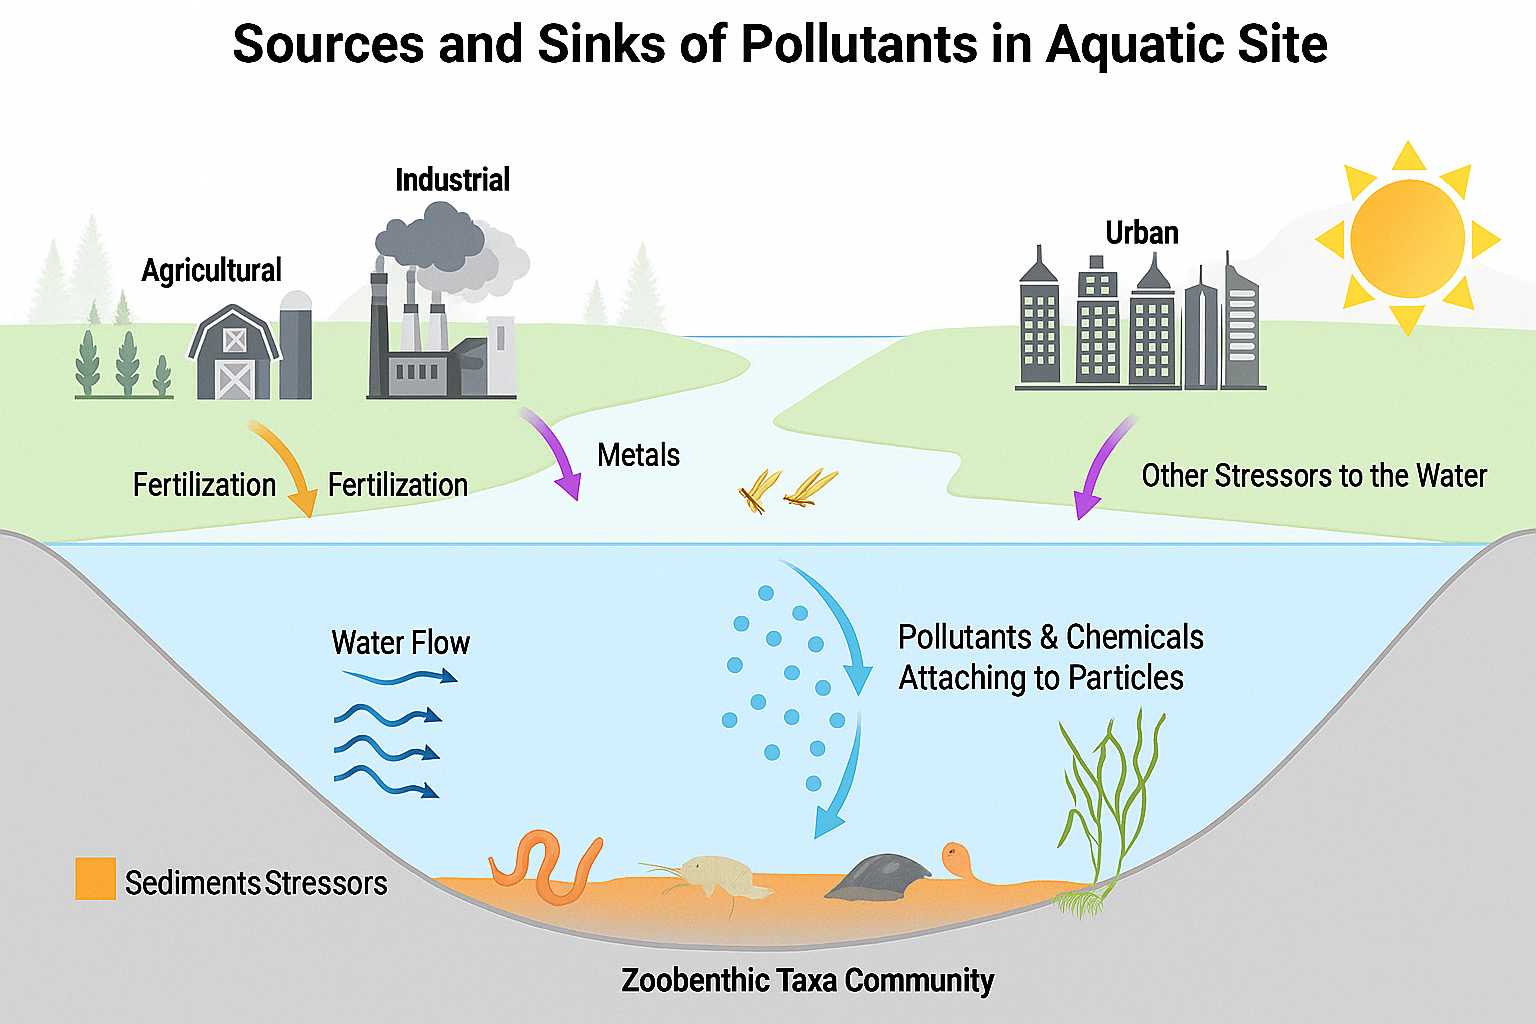
\includegraphics[width=0.9\textwidth]{../results/ideas_visualization/introduction_study_system.png}
    \caption{\textit{Overview of how zoobenthic communities live under both sediment contamination and natural environmental conditions, 
    and may respond to these external changes. 
    (Base template adapted from Selvi \textit{et al.} (2019) \cite{Selvi2019}, originally created and shared on \textbf{BioRender}. 
    Modified by Feng Gu using \textbf{Sora2} with text-based prompts.)}}
    \label{fig:introduction_study_system}

\end{figure}